\documentclass[12pt,a4paper]{article}
\usepackage[utf8]{inputenc}
\usepackage{amsmath}
\usepackage{amsfonts}
\usepackage{amssymb}
\usepackage{graphicx} % for figure
\usepackage[font=footnotesize]{caption}
\usepackage{subcaption}  % for subfigure
\usepackage{float}
\usepackage{indentfirst} % indent first line after section title
\usepackage{placeins} %FloatBarrier
\usepackage{afterpage}
\usepackage{numprint} % round numbers
\usepackage{siunitx} % round numbers
\usepackage{booktabs}  % nice looking tables

\author{Joao Guilherme Caldas Steinstraesser \\ José Galaz}
\title{Inriamericwaves \\ Report of activities - March-May/16}

\bibliographystyle{abbrv}

\captionsetup[subfigure]{labelformat=parens,labelsep=space}

%% Commands
\newcommand{\der}[1]{\partial_{#1}}
\renewcommand{\epsilon}{\varepsilon}

\renewcommand{\th}{\tilde{h}}
\newcommand{\tu}{\tilde{u}}

\newcommand{\lh}{\overline{h}}
\newcommand{\lu}{\overline{u}}

\newcommand{\opT}{\mathcal{T}}
\newcommand{\opQ}{\mathcal{Q}}
\newcommand{\opIT}{I + \opT}
\newcommand{\opIhT}{I + h\opT\frac{1}{h}}

\newcommand{\Atwo}[2]{\left( \begin{array}{c} #1 \\ #2  \end{array} \right)}

\newcommand{\laplinv}{\mathcal{L}^{-1}}

\begin{document}
\maketitle

\newpage
\tableofcontents

\newpage
\section{Study of Transparent Boundary Conditions in splitting methods}

\indent As an introduction for the future application of the Transparent Boundary Conditions in splitting methods, for the resolution of the wave propagation models studied in this project, we will present in this section a simple one-dimensional case, for which we will implement and qualitatively validate our proposed method. The idea is to verify if imposing independent boundary conditions for each step of the splitting method provides a good approximation for the TBCs.

\indent After this initial propose, we will work in the numerical experiment presented in \cite{halpern1986}. In this paper, approximate TBCs are implemented for a linear advection-diffusion equation with one time-dependent boundary condition, solved with a full method. Therefore, we will implement the tests described in the paper, in order to obtain the same results and compare with the solutions of the methods that we will propose.  

\subsection{Linear advection-diffusion equation}

\indent We seek to solve here the problem

\begin{equation}
	\label{eq:LinearAdvDiffEq}
	\begin{cases}
	u_t + au_x - \epsilon u_{xx} = 0, \ \ x \in \Omega = [0,1], \ \ t \ge 0  , \ \ a \in \mathbb{R}, \ \ \epsilon > 0 \\
	u(0,x) = u_0(x) = e^{-{\frac{(x-0.5)}{0.01}}^2} \\
	\text{+ boundary conditions} 		
	\end{cases} 
\end{equation}

\indent In order to focus our analysis in only one of the two boundaries, we will consider $a = 1$ (so the wave travels to the right), and choose $\epsilon = $ such that the arrival of the wave to the right boundary occurs before the arrival of the diffused solution to the left one. We will compare the results obtained with different methods :

\paragraph{Splitting method} :  The splitting method proposed here leads, in each time step $[t_n,t_{n+1}]$, to the resolution of the linear advection equation and the heat equation :

\begin{equation}
	\label{eq:operatorsSplitting}
	\begin{cases}
		L_a(v) = v_t + av_x  = 0, \ \ v^n = u^n, \ \ t \in [t_n,t_{n+1}] \\
		L_d(w) = w_t - \epsilon w_{xx} = 0, \ \ w^n = v^{n+1}, \ \ t \in [t_n,t_{n+1}]  \\
		u^{n+1} = w^{n+1}
	\end{cases}	
\end{equation}

\indent Both equations will be solved with Finite Difference methods. In the case of the linear advection, it will be an explicit backward method, with an homogeneous Dirichlet condition on the left boundary :

\begin{equation}
	\begin{cases}
		u_i^{n+1} = u_i^n - a\Delta t \frac{u_i^n - u_{i-1}^n}{\Delta x}, \ \ i = 1,...,N \\
		u_0^{n+1} = 0
	\end{cases}
\end{equation}

\indent For the heat equation, we will use the Crank-Nicolson method (semi-implicit), with homogeneous Neumann conditions in both boundaries :

\begin{equation}
\begin{cases}
\frac{u_i^{n+1}-u_i^{n}}{\Delta t} - \epsilon \frac{1}{2} \left( \frac{u_{i-1}^{n+1} - 2u_i^{n+1} + u_{i+1}^{n+1}}{\Delta x^2}  + \frac{u_{i-1}^{n} - 2u_i^{n} + u_{i+1}^{n}}{\Delta x^2} \right) = 0 \\
u_1^{n+1} = u_0^{n+1} \\
u_{N}^{n+1} = u_{N-1}^{n-1} 
\end{cases}
\end{equation}

\paragraph{Full equation} In order to compare with the results of the splitting method, we implemented a resolution of the full linear advection-diffusion equation, also with the Crank-Nicolson method, with an explicit discretization of the advection term : 

\begin{equation}
\begin{cases}
\frac{u_i^{n+1}-u_i^{n}}{\Delta t}  + a\frac{u_i^n - u_{i-1}^n}{\Delta x} - \epsilon \frac{1}{2} \left( \frac{u_{i-1}^{n+1} - 2u_i^{n+1} + u_{i+1}^{n+1}}{\Delta x^2}  + \frac{u_{i-1}^{n} - 2u_i^{n} + u_{i+1}^{n}}{\Delta x^2} \right) = 0 \\
		u_0^{n+1} = 0 \\
		B_j(u_n^{n+1}) = 0
\end{cases}
\end{equation}

\indent The boundary conditions $B_j$ are the approximate boundary conditions proposed in \cite{halpern1986}, where $j$ indicates the order of a Taylor expansion of the solutions of the characteristic equation obtained when solving  \ref{eq:LinearAdvDiffEq} in the Fourier space. We implemented here the zero and first order approximations:

\begin{equation}
	B_0 = u_x = 0 \implies u_N^{n+1} - u_{N-1}^{n+1} = 0
\end{equation}

\begin{equation}
	B_1 = u_t + u_x = 0 \implies \frac{u_N^{n+1} - u_N^{n}}{\Delta t} - \frac{u_N^{n+1} - u_{N-1}^{n+1}}{\Delta x} = 0
\end{equation}

\indent We notice that $B_0$ corresponds to an homogeneous Neumann boundary condition.

\indent We show in the figure \ref{fig:firstCase} some snapshots of the computed solutions. We compare them with a referential solution, which was computed with the full equation, using the TBC $B_1$ and in a larger domain ($\Omega_{ref} = [0,2]$). The choice of the boundary condition may not have an influence over the comparison that we intend to do here, because we will study the solution near the boundary $x=1$, which is far enough of the boundary in the referential domain.

\noindent\begin{minipage}{\textwidth} 
	\begin{minipage}{.5\textwidth} 
		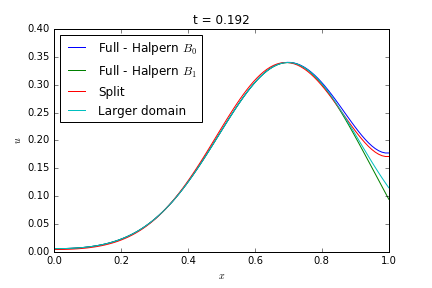
\includegraphics[scale=.48]{figures/firstCase1.png}	
		\captionof{subfigure}{Solution in the whole domain}
	\end{minipage}
	\begin{minipage}{.5\linewidth}
		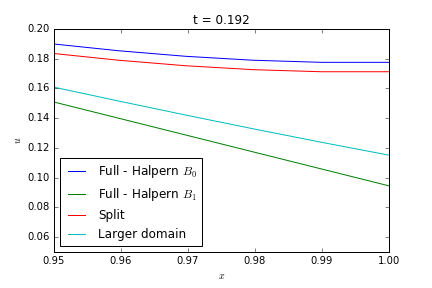
\includegraphics[scale=.48]{figures/firstCase1Detail.png}	
		\captionof{subfigure}{Detail  - right boundary}
	\end{minipage}
	\begin{minipage}{.5\textwidth} 
		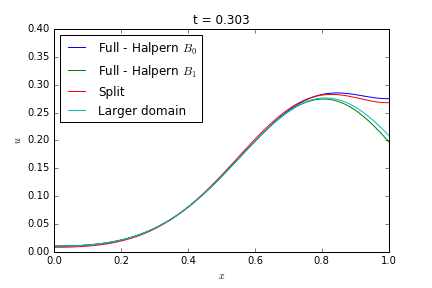
\includegraphics[scale=.48]{figures/firstCase2.png}	
		\captionof{subfigure}{Solution in the whole domain}
	\end{minipage}
	\begin{minipage}{.5\linewidth}
		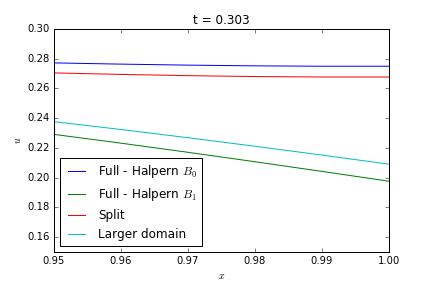
\includegraphics[scale=.48]{figures/firstCase2Detail.png}	
		\captionof{subfigure}{Detail  - right boundary}
	\end{minipage}
	\begin{minipage}{.5\textwidth} 
		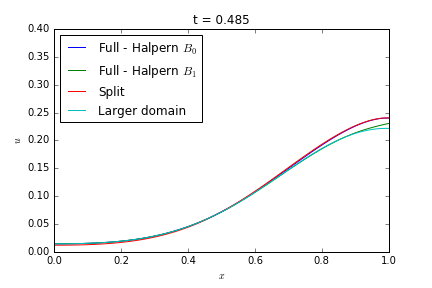
\includegraphics[scale=.48]{figures/firstCase3.png}	
		\captionof{subfigure}{Solution in the whole domain}
	\end{minipage}
	\begin{minipage}{.5\linewidth}
		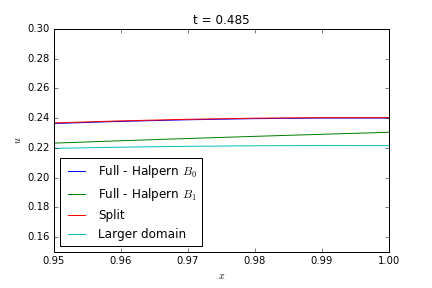
\includegraphics[scale=.48]{figures/firstCase3Detail.png}	
		\captionof{subfigure}{Detail  - right boundary}
	\end{minipage}
	\captionof{figure}{Results in different instants for the linear advection-diffusion equation, computed with a splitting method (in red) or full methods (in dark blue and green, with different approximate TBCs); also compared with a referential solution. \label{fig:firstCase}}
\end{minipage}

\indent The results of the figure \ref{fig:firstCase} shows that, compared with the referential solution, the condition $B_1$ provides a better approximation for the TBC. The full equation with $B_0$ and the splitting method provides similar but worse result, even though they qualitatively allows the solution to exit the domain without notable influence of the boundary.

\subsection{Numerical experiment realized in \cite{halpern1986}}

\indent In order to make a deeper study of the boundary conditions in splitting methods, we will implement the numerical experiment presented in \cite{halpern1986} and compare it with the solution of the splitted equation.

\indent This numerical experiment consists in the same linear advection-diffusion equation, but with zero initial conditions and a time-dependent boundary condition imposed on the left boundary :

\begin{equation}
	\label{eq:halpernProblem}
	\begin{cases}
	u_t + u_x - u_{xx} = 0, \ \ x \in \Omega = [0,1], \ \ t \ge 0  \\
	u(0,x) = 0, \ \ x \in \Omega \\
	u(t,0) = \frac{sin t}{\sqrt{t^2+1}} \\
	\text{+ right boundary conditions} 		
	\end{cases} 
\end{equation}

\indent Similarly to what we did in the previous section, \cite{halpern1986} considers a referential solution computed in the domain $
\Omega_{ref} = [0,2]$. In order to validate our implementation, we will repeat some tests presented in the paper: 

\begin{itemize}
	\item Full equation with right boundary condition $B_0$;
	\item Full equation with right boundary condition $B_1$;
	\item Transport equation (i.e, ignoring the diffusive term).
\end{itemize}

\indent We will also solve the equation using several splitting methods.  Recalling the operators defined in \eqref{eq:operatorsSplitting}, and introducing a superscript denoting the time interval in which the operator is solved, we will solve, for each time step

\begin{itemize}
	\item $L_d^{\Delta t}(L_a^{\Delta t}(u)) = 0$;
	\item $L_a^{\Delta t}(L_d^{\Delta t}(u)) = 0$;
	\item $L_a^{\Delta t/2}(L_d^{\Delta t}(L_a^{\Delta t/2}(u))) = 0$;
\end{itemize}

\noindent\begin{minipage}{\textwidth} 
	\begin{minipage}{.5\textwidth} 
		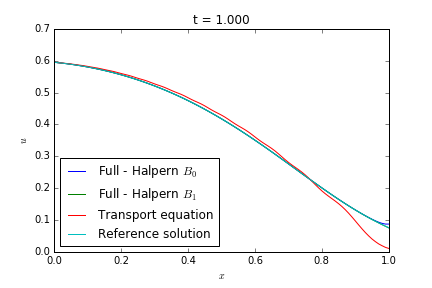
\includegraphics[scale=.48]{figures/secondCase1A.png}	
		\captionof{subfigure}{Solution in the whole domain}
	\end{minipage}
	\begin{minipage}{.5\linewidth}
		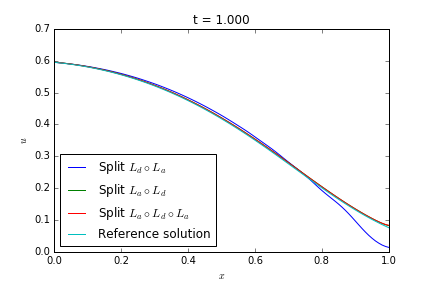
\includegraphics[scale=.48]{figures/secondCase1B.png}	
		\captionof{subfigure}{Solution in the whole domain}
	\end{minipage}
	\begin{minipage}{.5\textwidth} 
		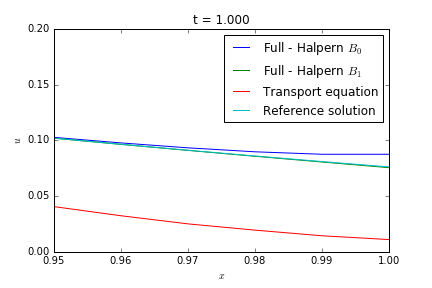
\includegraphics[scale=.48]{figures/secondCase1ADetail.png}	
		\captionof{subfigure}{Detail - right boundary}
	\end{minipage}
	\begin{minipage}{.5\linewidth}
		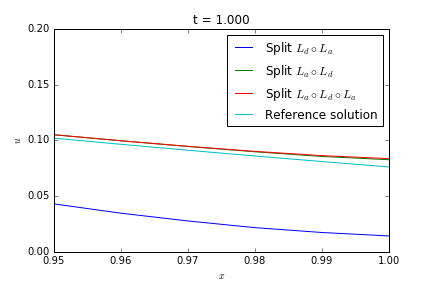
\includegraphics[scale=.48]{figures/secondCase1BDetail.png}	
		\captionof{subfigure}{Detail - right boundary}
	\end{minipage}
	\captionof{figure}{Results in $t=1$  for the numerical experiment in \cite{halpern1986}, computed with several methods and boundary conditions. \label{fig:secondCase}}
\end{minipage}

\indent Also as done in \cite{halpern1986}, we compute for each time step the error on the boundary, $e^n = u^n_N - (u_{ref})^n_N$, as shown in the figure \ref{fig:secondCaseErrors}

\noindent\begin{minipage}{\textwidth} 
	\begin{minipage}{.5\textwidth} 
		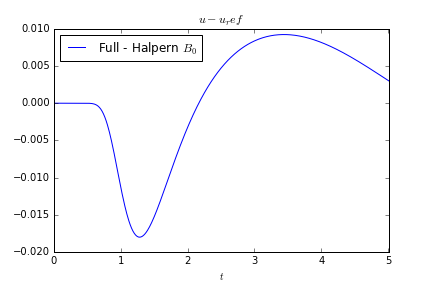
\includegraphics[scale=.48]{figures/errFullB0.png}	
		\captionof{subfigure}{Full equation with boundary condition $B_0$}
	\end{minipage}
	\begin{minipage}{.5\textwidth} 
		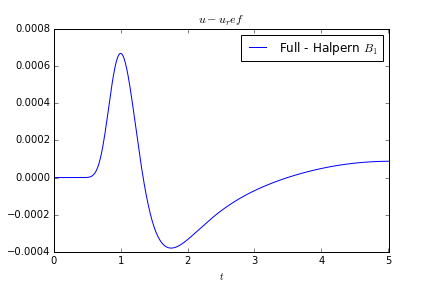
\includegraphics[scale=.48]{figures/errFullB1.png}	
		\captionof{subfigure}{Full equation with boundary condition $B_1$}
	\end{minipage}
	\begin{minipage}{.5\textwidth} 
		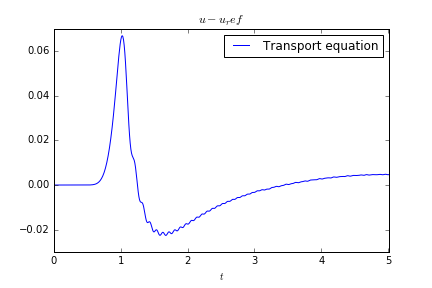
\includegraphics[scale=.48]{figures/errTransport.png}	
		\captionof{subfigure}{Transport equation}
	\end{minipage}
	\begin{minipage}{.5\textwidth} 
		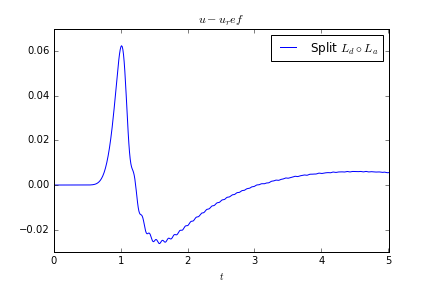
\includegraphics[scale=.48]{figures/errSplitA.png}	
		\captionof{subfigure}{Splitting  $L_d \circ L_a$}
	\end{minipage}
	\begin{minipage}{.5\textwidth} 
		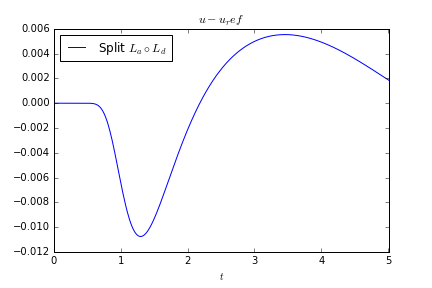
\includegraphics[scale=.48]{figures/errSplitB.png}	
		\captionof{subfigure}{Splitting  $L_a \circ L_d$}
	\end{minipage}
	\begin{minipage}{.5\textwidth} 
		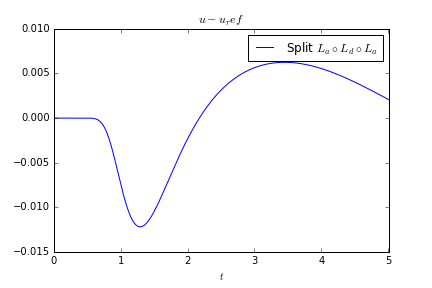
\includegraphics[scale=.48]{figures/errSplitC.png}	
		\captionof{subfigure}{Splitting  $L_a \circ L_d \circ L_a$}
	\end{minipage}
	\captionof{figure}{ Evolution of the error $e^n = u^n_N - (u_{ref})^n_N$ for each method implemented \label{fig:secondCaseErrors}}
\end{minipage}
\section{Derivation and approximation of Transparent Boundary Conditions for the linearized KdV equation}

\indent Two main objectives motivate the work developed in this section : firstly, we want to present the usual derivation of Transparent Boundary Conditions in the case of linearized problems; and secondly, after obtaining analytical expressions for the TBCs (which in general have a too much expensive application), we will propose, optimize and test approximations for them.

\subsection{Description of the TBCs}

\indent The derivation of the TBCs is based on \cite{besse2015} . We will consider the formulation for the continuous version of the homogeneous and linearized KdV equation :

\begin{equation}
\label{eq:kdv}
u_t + U_1u_x + U_2u_{xxx} = 0, \ \ U_1 \in \mathbb{R}, \ \ U_2 > 0
\end{equation}

\indent Denoting by $\laplinv$ the inverse Laplace transform, the TBCs are

\begin{equation}
\label{eq:TBC}
    \begin{cases}
        u(t,a) - U_2 \laplinv \left( \frac{\lambda_1(s)^2}{s} \right) * u_x(t,a) - U_2 \laplinv \left( \frac{\lambda_1(s)}{s} \right) * u_{xx}(t,a) = 0 \\
        u(t,b) - \laplinv \left( \frac{1}{\lambda_1(s)^2} \right) * u_{xx}(t,b) = 0 \\
        u_x(t,b) - \laplinv \left( \frac{1}{\lambda_1(s)} \right) * u_{xx}(t,b) = 0 
    \end{cases}
\end{equation}

\noindent where $[a,b]$ is the computational physical domain, $s \in \mathbb{C}$ is the Laplace frequency and $\lambda_1$ is one of the roots of the cubic characteristic equation obtained when solving \eqref{eq:kdv} in the Laplace space.

\indent We firstly notice that we can rewrite \eqref{eq:TBC} as

\begin{equation}
\label{eq:TBC2}
    \begin{cases}
        u(t,a) - U_2 \laplinv \left( \frac{\lambda_1(s)^2}{s} \hat{u}_x(t,s) \right)  - U_2 \laplinv \left( \frac{\lambda_1(s)}{s}  \hat{u}_{xx}(t,s) \right) = 0 \\
        u(t,b) - \laplinv \left( \frac{1}{\lambda_1(s)^2}   \hat{u}_{xx}(t,s) \right) = 0 \\
        u_x(t,b) - \laplinv \left( \frac{1}{\lambda_1(s)}   \hat{u}_{xx}(t,s) \right) = 0 
    \end{cases}
\end{equation}

\noindent where $\hat{u}$ is the Laplace transform of $u$.

\indent In the case of pure dispersion ($U_1 = 0$ and $U_2 = 1$), $\lambda$ is written as

$$ \label{eq:lambda} \lambda(s) = -\sqrt[3]{s} $$

\indent So, from \eqref{eq:lambda} we can write

\begin{equation}
    \label{eq:lambda2}
    \frac{\lambda}{s} = \frac{\lambda}{-\lambda^3} = -\frac{1}{\lambda^2} \\ 
    \frac{\lambda^2}{s} = \frac{\lambda^2}{-\lambda^3} = -\frac{1}{\lambda} \\
\end{equation}

\indent In the sequence, we will always consider this case ($U_1 = 0$ and $U_2 = 1$).



\subsection{Approximation of the TBCs}

\subsubsection{Approximation using a constant polynomial}

\indent In a first moment, we will approximate $\frac{\lambda^2}{s}$ by a constant polynomial $P_0(s) = c$. Therefore, from (\ref{eq:lambda2}) we get

\begin{equation}
    \frac{\lambda^2}{s} = c \\
    \frac{\lambda}{s} = -c^2 \\
    \frac{1}{\lambda_1(s)^2} = c^2 \\
    \frac{1}{\lambda_1(s)} = -c
\end{equation}

\noindent and replacing in (\ref{eq:TBC2}) and considering the linearity of the Laplace transform : 

\begin{equation}
\label{eq:TBC3}
    \begin{cases}
        u(t,a) - cU_2 u_x(t,a)  + c^2 U_2    u_{xx}(t,s) = 0 \\
        u(t,b) - c^2    \hat{u}_{xx}(t,s) = 0 \\
        u_x(t,b) + c u_{xx}(t,s)= 0 
    \end{cases}
\end{equation}

\indent Using finite difference approximations and considering different constants $c_L and c_R$ for the left and the right boundaries, (\ref{eq:TBC3}) is discretized as

\begin{equation}
\label{eq:TBC4}
    \begin{cases}
        u_0 - c_LU_2 \frac{u_1 - u_0}{\Delta x}  + c_L^2 U_2 \frac{u_0 -2u_1 + u_2}{\Delta x^2} = 0 \\
        u_N - c_R^2    \frac{u_N -2u_{N-1} + u_{N-2}}{\Delta x^2} = 0 \\
        \frac{u_N - u_{N-1}}{\Delta x}  + c_R^2    \frac{u_N -2u_{N-1} + u_{N-2}}{\Delta x^2} = 0 
    \end{cases}
\end{equation}



\subsubsection{Approximation using a linear polynomial}


\indent Similarly to the case presented above, we will approximate $\frac{\lambda^2}{s}$ by a linear polynomial $P_1(s) = ds + c$. Therefore,

\begin{equation}
    \frac{\lambda^2}{s} = ds + c \\
    \frac{\lambda}{s} = -(ds + c )^2 \\
    \frac{1}{\lambda_1(s)^2} = (ds + c )^2 \\
    \frac{1}{\lambda_1(s)} = -(ds + c )  
\end{equation}

\indent Thus, the inverse Laplace transforms in (\ref{eq:TBC2}) reads :

\begin{equation}
	\begin{split}
    \mathcal{L}^{-1} \left( \frac{\lambda^2}{s} \hat{u}_x(t,s) \right) = & \mathcal{L}^{-1} \left[ (ds+c) \hat{u}_x(t,s) \right] = \\
    			 & d\mathcal{L}^{-1} \left[ \hat{u}_{xt}(t,s) \right] + c \mathcal{L}^{-1} \left[ \hat{u}_{x}(t,s) \right] =   du_{xt}(x,t) + cu_x(x,t) \\
    \mathcal{L}^{-1} \left( \frac{\lambda}{s} \hat{u}_{xx}(t,s) \right) = & \mathcal{L}^{-1} \left[ -(ds+c)^2 \hat{u}_{xx}(t,s) \right] =  -d^2u_{xxtt}(x,t) -2dcu_{xxt}(x,t) - c^2u_{xx}(x,t) \\
    \mathcal{L}^{-1} \left( \frac{1}{\lambda^2} \hat{u}_{xx}(t,s) \right) = & \mathcal{L}^{-1} \left[ (ds+c)^2 \hat{u}_{xx}(t,s) \right] =d^2u_{xxtt}(x,t) + 2dcu_{xxt}(x,t) + c^2u_{xx}(x,t) \\
    \mathcal{L}^{-1} \left( \frac{1}{\lambda} \hat{u}_{xx}(t,s) \right) = & \mathcal{L}^{-1} \left[ -(ds+c) \hat{u}_{xx}(t,s) \right] = -du_{xxt}(x,t) - cu_{xx}(x,t)
    \end{split}
\end{equation}

\indent Using finite differences and different coefficients $c_L,c_R$ and $d_L,d_R$ for the left and the right boundaries, these expressions can be approximated by

\begin{equation}
    \label{eq:FDorder2A}
    \begin{split}
    \mathcal{L}^{-1} \left( \frac{\lambda^2}{s} \hat{u}_x(t,s) \right) = & d_L \frac{ (u_x)_0^{n+1} - (u_x)_0^n}{\Delta t} + c_L (u_x)_0^{n+1} = \\
    			& \left( \frac{d_L}{\Delta t} + c_L \right) \left( \frac{u_1^{n+1} - u_0^{n+1}}{\Delta x}\right) - \frac{d_L}{\Delta t} \left( \frac{u_1^{n} - u_0^{n}}{\Delta x}\right)
    \end{split}
 \end{equation}
 
 \begin{equation}
     \label{eq:FDorder2B}
    \begin{split}
    \mathcal{L}^{-1} \left( \frac{\lambda}{s} \hat{u}_{xx}(t,s) \right) = & -d_L^2 \left( \frac{(u_{xx})_0^{n+1} - 2(u_{xx})_0^{n} + (u_{xx})_0^{n-1}}{\Delta t^2} \right) + \\
    			&  - 2d_Lc_L \left( \frac{(u_{xx})_0^{n+1} - (u_{xx})_0^{n}}{\Delta t} \right) - c_L^2 (u_{xx})_0^{n+1} = \\
    			& -\left( \frac{d_L^2}{\Delta t^2} + \frac{2d_Lc_L}{\Delta t} + c_L^2  \right) \left(  \frac{u_0^{n+1} - 2u_1^{n+1} + u_2^{n+1}}{\Delta x^2} \right) + \\
    			& \left( 2\frac{d_L^2}{\Delta t^2} + \frac{2d_Lc_L}{\Delta t}\right) \left(  \frac{u_0^{n} - 2u_1^n + u_2^{n}}{\Delta x^2} \right) - \frac{d_L^2}{\Delta t^2} \left(  \frac{u_0^{n-1} - 2u_1^{n-1} + u_2^{n-1}}{\Delta x^2} \right)
    \end{split}
 \end{equation}
     			
\begin{equation}
     \label{eq:FDorder2C}
         \begin{split}
    \mathcal{L}^{-1} \left( \frac{1}{\lambda^2} \hat{u}_{xx}(t,s) \right) = & \left( \frac{d_R^2}{\Delta t^2} + \frac{2d_Rc_R}{\Delta t} + c_R^2  \right) \left(  \frac{u_{N}^{n+1} - 2u_{N-1}^{n+1} + u_{N-2}^{n+1}}{\Delta x^2} \right) + \\
    			& - \left( 2\frac{d_R^2}{\Delta t^2} + \frac{2d_Rc_R}{\Delta t}\right) \left(  \frac{u_N^{n} - 2u_{N-1}^n + u_{N-2}^{n}}{\Delta x^2} \right) + \\
    			& \frac{d_R^2}{\Delta t^2} \left(  \frac{u_N^{n-1} - 2u_{N-1}^{n-1} + u_{N-2}^{n-1}}{\Delta x^2} \right)
    \end{split}
 \end{equation}
     			
\begin{equation}
     \label{eq:FDorder2D}
         \begin{split}
    \mathcal{L}^{-1} \left( \frac{1}{\lambda} \hat{u}_{xx}(t,s) \right) = & -d_R \frac{ (u_{xx})_0^{n+1} - (u_{xx})_0^n}{\Delta t} - c_R (u_{xx})_0^{n+1} =\\
    			& -\left( \frac{d_R}{\Delta t} + c_R \right) \left( \frac{u_N^{n+1} -2 u_{N-1}^{n+1} + u_{N-2}^{n+1}}{\Delta x^2}\right) + \frac{d_R}{\Delta t}\left( \frac{u_{N}^{n} - 2u_{N-1}^{n} + u_{N-2}^n}{\Delta x^2}\right)
    \end{split}
\end{equation}

\indent Then we use \eqref{eq:FDorder2A} - \eqref{eq:FDorder2D} in \eqref{eq:TBC2} to obtain the discrete TBCs :

\begin{equation}
	\begin{split}
    u_0^{n+1} - U_2\left( \frac{d_L}{\Delta t} + c_L \right) \left( \frac{u_1^{n+1} - u_0^{n+1}}{\Delta x}\right) + \\
     U_2\left( \frac{d_L^2}{\Delta t^2} + \frac{2d_Lc_L}{\Delta t} + c_L^2  \right) \left(  \frac{u_0^{n+1} - 2u_1^{n+1} + u_2^{n+1}}{\Delta x^2} \right) = \\
     -U_2\frac{d_L}{\Delta t}\left( \frac{u_1^{n} - u_0^{n}}{\Delta x}\right) + U_2 \left( 2\frac{d_L^2}{\Delta t^2} + \frac{2d_Lc_L}{\Delta t}\right) \left(  \frac{u_0^{n} - 2u_1^n + u_2^{n}}{\Delta x^2} \right) + \\
     - U_2 \frac{d_L^2}{\Delta t^2} \left(  \frac{u_0^{n-1} - 2u_1^{n-1} + u_2^{n-1}}{\Delta x^2} \right)
   \end{split}
\end{equation} 

\begin{equation}
	\begin{split}
    u_N^{n+1} - \left( \frac{d_R^2}{\Delta t^2} + \frac{2d_Rc_R}{\Delta t} + c_R^2  \right) \left(  \frac{u_{N}^{n+1} - 2u_{N-1}^{n+1} + u_{N-2}^{n+1}}{\Delta x^2} \right) =\\
     -\left( 2\frac{d_R^2}{\Delta t^2} + \frac{2d_Rc_R}{\Delta t}\right) \left(  \frac{u_N^{n} - 2u_{N-1}^n + u_{N-2}^{n}}{\Delta x^2} \right) + \frac{d_R^2}{\Delta t^2} \left(  \frac{u_N^{n-1} - 2u_{N-1}^{n-1} + u_{N-2}^{n-1}}{\Delta x^2} \right)
    \end{split}
\end{equation} 
   
\begin{equation}
	\begin{split}	
    \frac{u_N^{n+1} - u_{N-1}^{n+1}}{\Delta x} + \left( \frac{d_R}{\Delta t} + c_R \right) \left( \frac{u_N^{n+1} -2 u_{N-1}^{n+1} + u_{N-2}^{n+1}}{\Delta x^2}\right) = \\
      \frac{d_R}{\Delta t}\left( \frac{u_{N}^{n} - 2u_{N-1}^{n} + u_{N-2}^n}{\Delta x^2}\right)
    \end{split}
\end{equation}


\subsection{Numerical tests}

\indent In order to validate compare our approximation with the results obtained by Besse, we will solve the same numerical test presented in his paper : 

\begin{equation}
\label{eq:Num1}
 u_t + u_{xxx} = 0, \ \ x \in \mathbb{R}
\end{equation}

\begin{equation}
\label{eq:Num2}
 u(0,x) = e^{-x^2}, \ \ x \in \mathbb{R} 
\end{equation}

\begin{equation}
\label{eq:Num3}
 u \rightarrow 0, \ \ |x| \rightarrow \infty
\end{equation}

\indent The fundamental solution of (\ref{eq:Num1}) is

\begin{equation}
    E(t,x) = \frac{1}{\sqrt[3]{3t}}Ai\left(\frac{x}{\sqrt[3]{3t}} \right)
\end{equation}

\noindent where $Ai$ is the Airy function, and the exact solution for the problem (\ref{eq:Num1}) - (\ref{eq:Num3}) is

\begin{equation}
    u_{exact}(t,x) = E(t,x) * e^{-x^2}
\end{equation}

\indent The problem will be solved in the spatial domain $[-6,-6]$

\indent For a quantitative evaluation of the results, we computed the same errors defined in the paper of Besse et al. For each time step, we compute the relative error

$$e^n = \frac{\left\Vert u_{exact}^n - u_{computed}^n\right\Vert_2}{\left\Vert u_{exact}^n\right\Vert_2}$$

\noindent and, in the whole time interval :

$$ e_{Tm} = \max\limits_{0 < n < T_{max}} (e^n) $$

$$ e_{L2} = \sqrt{ \Delta t \sum_{n=1}^{T_{max}} (e^n)^2 } $$

\indent We also generate plottings and animations for the best and the worst solutions. In order to make a better comparison, in the definition of "worst solution" we ignored the ones for which the numerical computations diverged (following the arbitrary criteria $e_{L2} > 10$.

\indent Several tests will be made with different combinations of the coefficients in the polynomial approximation of $\frac{\lambda^2}{s}$. For the constant polynomial $P_0(s) = c$, we will optimize the parameters $(c_L,c_R)$. For the linear polynomial $P_1(s) = cs+d$, we will optimize the four parameters $(c_L,d_L,c_R,d_R)$, but in a first moment we will consider $c_L = c_R$ and $d_L = d_R$ and study the behavior of the approximation in only one of the boundaries.


\subsection{Introduction tests}

\indent In a first moment, we will execute the tests with the proposed TBCs for a small range of parameters $(c_L,c_R)$ (for the constant polynomial approximation) and $(c_L,c_R,d_L,d_R)$ (for the linear polynomial approximation).  We tested all the possible combinations between the values in $[-10,-1,-0.1,0,0.1,1,10]$. In the case of the linear polynomial approximation, in order to avoid large computations, we considered only the cases where $c_L = c_R$ and $d_L = d_R$.

\indent The objective of these initial tests is to see the general behavior of the proposed approximations and guide our next steps in this study. The tables \ref{tab:firstTestsP0} and \ref{tab:firstTestsP1} show the best results (concerning the error $e_{L2}$) for each one of the approximations; and the figures \ref{fig:firstTestsP0} and \ref{fig:firstTestsP1} show some snapshots comparing the best, the worst and the analytical solution. The choice of the worst solution does not consider the ones that "exploded".

	 \sisetup{round-mode=places}
\begin{center}
\begin{tabular}{c|c|S[round-precision=4,table-number-alignment =  left]}
	\multicolumn{1}{c|}{$c_L$}  & \multicolumn{1}{c|}{$c_R$} & \multicolumn{1}{r}{$e_{L2}$} \\
	\hline
	1.0 & 1.0 & 0.0946839239675 \\
	1.0 & 10.0 & 0.097288371204 \\
	1.0 & 0.1 & 0.0983932287563 \\
	1.0 & 0.0 & 0.0992063806502 \\
	1.0 & -10.0 & 0.099359192771 \\
	1.0 & -0.1 & 0.100021589665 \\
	1.0 &  -1. & 0.10159265619 \\
	10.0 & 1.0 & 0.347003021321 \\
	10.0 & 0.1 & 0.347379492262 \\
	10.0 & 0.0 & 0.347487945035
\end{tabular}
\captionof{table}{Best results (smallest $e_{L2}$) for the constant polynomial approximation \label{tab:firstTestsP0}}
\end{center}


	 \sisetup{round-mode=places}
\begin{center}
\begin{tabular}{c|c|S[round-precision=4,table-number-alignment =  left]}
	\multicolumn{1}{c|}{$d_L = d_R$}  & \multicolumn{1}{c|}{$c_L = c_R$} & \multicolumn{1}{r}{$e_{L2}$} \\
	\hline
	0. & 1.0 & 0.0946839239675 \\
	0.1 & 1.0 & 0.12341195 \\
	1.0 & 1.0 & 0.20031603 \\
	10.0 & 0.1 & 0.22037249 \\
	-10.0 & 0.1 & 0.23984486 \\
	10.0 & 1.0 & 0.27161158 \\
	-10.0 &  0.0 & 0.24800816\\
	-10.0 & 1.0 & 0.30039637 \\
	10.0 & 0.0 & 0.27213611 \\
	0.0 & 0.1 & 0.36740764
\end{tabular}
\captionof{table}{Best results (smallest $e_{L2}$) for the linear polynomial approximation \label{tab:firstTestsP1}}
\end{center}

\noindent\begin{minipage}{\textwidth} 
	\begin{minipage}{.5\textwidth} 
		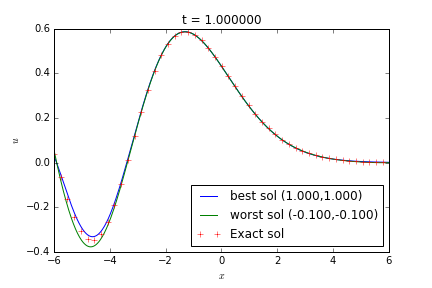
\includegraphics[scale=.48]{figures/TBCbesse/firstTestsP0Snap2.png}	
	\end{minipage}
	\begin{minipage}{.5\linewidth}
		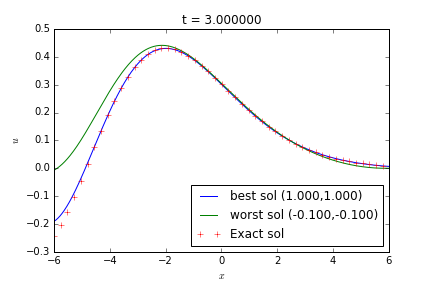
\includegraphics[scale=.48]{figures/TBCbesse/firstTestsP0Snap4.png}	
	\end{minipage}
	\captionof{figure}{Snapshots with the best and the worst solution in the case of the constant polynomial approximation \label{fig:firstTestsP0}}
\end{minipage}

\noindent\begin{minipage}{\textwidth} 
	\begin{minipage}{.5\textwidth} 
		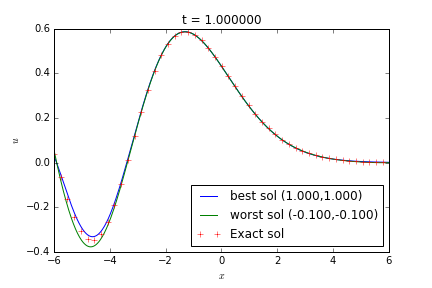
\includegraphics[scale=.48]{figures/TBCbesse/firstTestsP0Snap2.png}	
	\end{minipage}
	\begin{minipage}{.5\linewidth}
		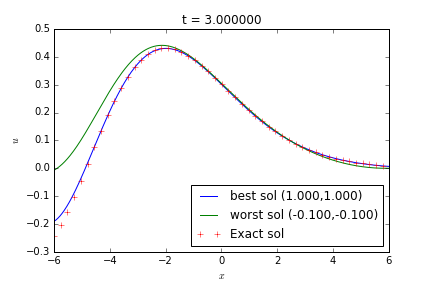
\includegraphics[scale=.48]{figures/TBCbesse/firstTestsP0Snap4.png}	
	\end{minipage}
	\captionof{figure}{Snapshots with the best and the worst solution in the case of the linear polynomial approximation \label{fig:firstTestsP1}}
\end{minipage}

\indent The results of the tables \ref{tab:firstTestsP0} and \ref{tab:firstTestsP1} and the figures \ref{fig:firstTestsP0} and \ref{fig:firstTestsP1} shows that using a higher-order polynomial approximation in the TBCs (which implies the existence of time derivative terms) does not improve the error of the numerical solution. In fact, the best solution was the one with $d_L = d_R = 0$, which leads to constant polynomial case. Additionally, The tests with $P_0$ shows that the solution is much more sensitive to the left than the right boundary, which is a consequence of the fact that the solution is practically constant and equal to zero in $L=6$, but shows great variations in $L=-6$.

\indent Therefore, in the following we will work only with the constant polynomial approximation, due to the better results that it provides and its simpler implementation.
\section{Application to a Domain Decomposition Method}

\indent The constant polynomial approximation of the Transparent Boundary Conditions, expressed by \ref{eq:TBC3}, will be applied to the implementation of a Domain Decomposition Method (DDM). Firstly, we will briefly describe the DDM that we will consider here, and after we will describe and test the incorporation of the proposed TBCs.

\subsection{The Schwarz Methods}

\indent The following description is based on \cite{Japhet2003}. Domain Decomposition Methods allow to decompose a domain $\Omega$ in multiple subdomains $\Omega_i$ (that can possibly overlap) and solve the problem in each one of them. Therefore, one must find functions that satisfies the PDE in each subdomain and that match on the interfaces. 

\indent The first DDM developed was the Schwarz method, which consists on an iterative method : in the case of a evolution problem, the solution  $u_i^{n,\infty}$, in each time step $t_n$ and each subdomain $\Omega_i$, is computed as the convergence of the solution obtained in each iteration, $u_i^{n,k}, \ \ k\geq 0$. There are two types of Schwarz methods, depending on the way that the boundary conditions on the interfaces are constructed for computing $u_i^{n,k}$

\indent We will consider her the additive Schwarz method (ASM), in which the boundary conditions are always constructed using the solution $u_j^{n,k-1}, \ \ j \neq i$ of the previous iteration in the other partitions of the domain. Therefore, in each interface between the domains $\Omega_i$ and $\Omega_j$, the boundary condition for the problem in $\Omega_i$ is

$$\mathcal{B}(u_i^{n,k+1}) = \mathcal{B}(u_j^{n,k})$$

\noindent where $\mathcal{B}$ denotes the operator of the TBC.

%\indent In the order hand, the multiplicative Schwarz method (MSM) uses always the most recent information for computing the interface boundary conditions. Therefore, if we consider a DDM with two subomains, $\Omega_1$ and $\Omega_2$,  they TBCs would be written (for example) as 

%$$\mathcal{B}(u_1^{n,k+1}) = \mathcal{B}(u_2^{n,k}) \\ \mathcal{B}(u_2^{n,k+1}) = \mathcal{B}(u_1^{n,k+1})$$

%\noindent for solving the problem in $\Omega_1$ and $\Omega_2$, respectively.

%\indent We will consider here only the ASM.In the following description, without lost of generality, we will consider a domain decomposed in two non-overlapping subdomains.

\indent Without loss of generality, in the following we will consider a domain decomposed in two non-overlapping subdomains.

\indent Evidently, the biggest challenge of the Schwarz methods is to define appropriate operators such that :

\begin{itemize}
\item The method shows a fast convergence
\item The solution $u_i$ in each subdomain $\Omega_i$ converges to $u|_{\Omega_1}$, i.e, the solution $u$ of the monodomain $\Omega$ restricted to $\Omega_1$
\end{itemize} 

\indent In fact, accordingly to \cite{Japhet2013}, the optimal additive Schwarz method is the one which uses the TBCs \ref{REFTBCMAY} as interface boundary conditions: with them, the method converges in two iterations, and no ASM can converge in less than two iterations.

\indent Nevertheless, as discussed previously in this report, the numerical implementation of the exact TBCs \ref{REFTBCMAY} are generally impractical, because they are non local in time. Therefore, one should use approximate TBCs, what will be done here in the sequence using the approximations proposed n the previous section.

\subsection{ASM with the approximate TBCs for the dispersive equation}

\indent The resolution of the dispersive equation with the Additive Schwarz method, using the constant polynomial approximation for the TBCs, is written as

\begin{equation}
    \label{eq:problemDDM1}
    \begin{cases}
        (u_1^{n,k+1})_t + (u_1^{n,k+1})_{xxx} = 0 , \ \ x \in \Omega_1, \ \ t \leq 0\\
        u_1^{n,0} = u_1^{n-1,\infty} , \ \ x \in \Omega_1 \\
        \Upsilon_1^{c_L^*}(u_1^{n+1,k+1},-L) = 0, \\ 
        \Theta_2^{c_R^*}(u_1^{n+1,k+1},0) = \Theta_2^{c_R^*}(u_2^{n,k},0) , \\
        \Theta_3^{c_R^*}(u_1^{n+1,k+1},0) = \Theta_3^{c_R^*}(u_2^{n,k},0)
     \end{cases}
\end{equation}

\begin{equation}
    \label{eq:problemDDM2}
    \begin{cases}
        (u_2^{n,k+1})_t + (u_2^{n,k+1})_{xxx} = 0 , \ \ x \in \Omega_2, \ \ t \leq 0\\
        u_2^{n,0} = u_2^{n-1,\infty} , \ \ x \in \Omega_2 \\
        \Theta_1^{c_L^*}(u_2^{n+1,k+1},0) = \Theta_1^{c_L^*}(u_1^{n,k},0) \\
        \Upsilon_2^{c_R^*}(u_2^{n+1,k+1},L) = 0 \\
        \Upsilon_3^{c_R^*}(u_2^{n+1,k+1},L) = 0
     \end{cases}
\end{equation}

\indent where $ \Upsilon_i, \ \ i=1,2,3$, are the boundary conditions on the external boundaries (i.e, in the intersection of the monodomain boundaries and the subdomain boundaries). These external BCs are independent of the interface BCs. Here, we will consider $\Upsilon_1 = \Theta_1^{1.0}$, $\Upsilon_2 = \Theta_2^{0.0}$ and $\Upsilon_3 = \Theta_3^{0.0}$, which gives

\begin{gather}
	\Upsilon_1(u,x) = u - u_x + u_{xx} \\
	\Upsilon_2(u,x) = 0 \\
	\Upsilon_3(u,x) = 0 \\
\end{gather}

\indent This choice was made based on the easy implementation and the good results provided by the coefficients $c_L = 1.0$ and $c_R = 0.0$ in approximating the analytical solution in $\Omega$ (as shown in the table \ref{tab:firstTestsP0}). Nevertheless,it does not have much importance in the study that we will done in the following paragraphs. In fact, our purpose is to study exclusively the behavior of the DDM implemented here; therefore, all the results must be compared to a referential solution $u_{ref}$, that can be simply the numerical solution of the monodomain problem. The only restriction for an appropriate study is that the external BCs for computing $u_{ref}$ must be same as $\Upsilon_i, \ \ i=1,2,3$.

\subsection{Error in the converged solution}

\indent When using approximate TBCs in the ASM, one should guarantee that the converged solutions $u_1,u_2$ satisfies the same equation as the solution $u_{ref}$ of the monodomain problem. In the following paragraphs, we show that this property is not verified by the method \eqref{eq:problemDDM1} - \eqref{eq:problemDDM2} proposed here. Based on that, we will be able to propose corrections for it.


\subsubsection{Study of the error in the DDM method for the dispersion equation}

\indent Now we will apply a similar idea to study the error of the Domain Decomposition Method that we proposed for the dispersive equation. As mentioned above, we will focus exclusively on the error produced by DDM, independently of the other possible components of the error compared to the exact solution for the example (external boundary conditions, error accumulation over the time steps). Therefore, all the following study will be made considering the execution of the method over only one time step, allowing us to use a clearer notation for the solution : $u_j^i$, where $i$ indicates the subdomain $\Omega_i$ and $j$ indicates the spatial discrete position. In the cases where the iterative process is take in account, we will add the superscript $k$ to indicate the iteration.

\indent For the interior points of each one of the domains, we will consider a second order spatial discretization of the equation (\ref{eq:linearizedKdV}).

\begin{equation}
    \label{eq:FDdiscretization}
    \frac{u_j^i - \alpha_j^i}{\Delta t} + \frac{-\frac{1}{2}u_{j-2}^i + u_{j-1}^i - u_{j+1}^i + \frac{1}{2}u_{j+2}^i }{\Delta x ^3} = 0
\end{equation}

\indent for $j=2,...,N-2$ in the case $i=1$; for $j=N+2,...,2N-2$ in the case $i=2$; and for $j=2,...,2N-2$ in the case $i=ref$. In the above expression, $\alpha_j^i$ is a given data (for example, the converged solution in the previous time step).

\indent For the points near the boundaries, we use second order uncentered discretizations or the appropriate TBCs. We will focus here on the interface point $x_N$. Thus, in the resolution of the problem in $\Omega_1$, two interface boundary conditions are imposed (corresponding to $\Theta_2$ and $\Theta_3$), so the solutions $u_{N-1}^1$ and $u_N^1$ are computed using the equations

\begin{equation}
	\begin{aligned}
    \label{eq:TBCsIterOmega1A}
    && 				&\Theta_2^{c_R}(u_N^1) = \Theta_2^{c_R}(u_N^2) \implies \\ 
    && \implies & u_N^1 - c_R^2 \frac{u_N^1 - 2u_{N-1}^1 + u_{N-2}^1}{\Delta x^2} = u_N^2 - c_R^2 \frac{u_N^2 - 2u_{N+1}^2 + u_{N+2}^2}{\Delta x^2} 
    \end{aligned}
\end{equation}

\begin{equation}
	\begin{aligned}
    \label{eq:TBCsIterOmega1B}
    && 			   & \Theta_3^{c_R}(u_N^1) = \Theta_3^{c_R}(u_N^2) \implies \\
    && \implies & \frac{u_N^1 - u_{N-1}^1}{\Delta x} + c_R \frac{u_N^1 - 2u_{N-1}^1 + u_{N-2}^1}{\Delta x^2} = \frac{u_{N+1}^2 - u_{N}^2}{\Delta x} + c_R \frac{u_N^2 - 2u_{N+1}^2 + u_{N+2}^2}{\Delta x^2}
    \end{aligned}
\end{equation}

\indent In the resolution of the problem in $\Omega_2$, only one interface boundary condition is used (corresponding to $\Theta_1$) :

\begin{equation}
	\begin{aligned}
    \label{eq:TBCsIterOmega2}
    && 				&\Theta_3^{c_L}(u_N^2) = \Theta_3^{c_L}(u_N^1) \implies \\ 
    && \implies & u_N^2 - c_L \frac{u_{N+1}^2 - u_{N}^2}{\Delta x} + c_L^2 \frac{u_N^2 - 2u_{N+1}^2 + u_{N+2}^2}{\Delta x^2}  =\\
    && 				& u_N^1 - c_L \frac{u_{N}^1 - u_{N-1}^1}{\Delta x} + c_L^2 \frac{u_N^1 - 2u_{N-1}^1 + u_{N-2}^1}{\Delta x^2}
    \end{aligned}
\end{equation}

\indent In the convergence, \eqref{eq:TBCsIterOmega1A} to\eqref{eq:TBCsIterOmega2} gives respectively

\begin{equation}
    \label{eq:TBCsCVOmega1A}
\begin{aligned}
    && 			    &u_N^* - c_R^2 \frac{u_N^* - 2u_{N-1}^* + u_{N-2}^*}{\Delta x^2} = u_N^* - c_R^2 \frac{u_N^* - 2u_{N+1}^* + u_{N+2}^*}{\Delta x^2} \implies  \\
    && \implies & 2c_R^2 \frac{-\frac{1}{2}u_{N-2}^* + u_{N-1}^* - u_{N+1}^* + \frac{1}{2}u_{N+2}^* }{\Delta x^2} = 0
    \end{aligned}
    \end{equation}
    
\begin{equation}
    \label{eq:TBCsCVOmega1B}
\begin{aligned}
    &&             &\frac{u_N^* - u_{N-1}^*}{\Delta x} + c_R \frac{u_N^* - 2u_{N-1}^* + u_{N-2}^*}{\Delta x^2} = \\
    && 			   &\frac{u_{N+1}^* - u_{N}^*}{\Delta x} + c_R \frac{u_N^* - 2u_{N+1}^* + u_{N+2}^*}{\Delta x^2} \implies \\
    && \implies & -\frac{u_{N-1}^* - 2 u_{N}^* + u_{N+1}^*}{\Delta x} - 2c_R\frac{-\frac{1}{2}u_{N-2}^* + u_{N-1}^* - u_{N+1}^* + \frac{1}{2}u_{N+2}^* }{\Delta x^2} = 0 
\end{aligned}
\end{equation}

\begin{equation}
    \label{eq:TBCsCVOmega2}
\begin{aligned}
   && 					&	 u_N^* -  c_L\frac{u_{N+1}^* - u_{N}^*}{\Delta x} + c_L^2 \frac{u_{N}^* - 2u_{N+1}^* + u_{N+2}^*}{\Delta x^2} = \\ 
   && 					& u_N^* -  c_L\frac{u_{N}^* - u_{N-1}^*}{\Delta x} + c_L^2 \frac{u_{N}^* - 2u_{N-1}^* + u_{N-2}^*}{\Delta x^2} \implies \\
	&&  \implies	    & -c_L\frac{u_{N-1}^* - 2 u_{N}^* + u_{N+1}^*}{\Delta x} + 2c_L^2\frac{-\frac{1}{2}u_{N-2}^* + u_{N-1}^* - u_{N+1}^* + \frac{1}{2}u_{N+2}^* }{\Delta x^2} = 0 
\end{aligned}
\end{equation}

\indent Therefore, we can see that, the converged solution of the DDM method satisfies the same equation as the reference solution in all the points $x_j \in \Omega_1$, except in $x_{N-1}$ and $x_N$ (for the problem solved in $\Omega_1$) and in $x_N$ (for the problem solved in $\Omega_2$) . For example, it's easy to verify that \eqref{eq:TBCsCVOmega1A} differ from \eqref{eq:FDdiscretization} by a $O(\Delta x)$ term :

\begin{equation}
    \label{eq:diffEquations}
    \begin{aligned}
    2\Delta x c_R^2\left( \frac{u_N^* - \alpha_N^*}{\Delta t} + \frac{-\frac{1}{2}u_{N-2}^* + u_{N-1}^* - u_{N+1}^* + \frac{1}{2}u_{N+2}^* }{\Delta x ^3} \right) - \\
    \left( 2c_R^2 \frac{-\frac{1}{2}u_{N-2}^* + u_{N-1}^* - u_{N+1}^* + \frac{1}{2}u_{N+2}^* }{\Delta x^2} \right) =  2\Delta x c_R^2 \frac{u_N^* - \alpha_N^*}{\Delta t}
    \end{aligned}
\end{equation}

\paragraph{Numerical verification of the error}

\indent The problem \eqref{eq:problemDDM1} - \eqref{eq:problemDDM2} was solved until the convergence with 5 different uniform spatial discretizations, over one time step (in the interval $[0,\Delta t]$). In each case, the adopted referential solution $u^{ref}$ was the monodomain problem, solved with the same mesh size. Two errors were computed : 

\begin{equation}
	e^{N,\Omega_1\bigcap \Omega_2} = |u^{ref}_N - u^{1}_N|
\end{equation}

\begin{equation}
	e^{N,\Omega} = ||u^{ref}_N - u^{1,2}_N||_2 = \sqrt{dx}\sqrt{\sum_{j=0}^N{(u^{ref}_j - u^{1}_j)^2 } + \sum_{j=N}^{2N}{(u^{ref}_j - u^{2}_j)^2 } }
\end{equation}

\noindent corresponding respectively to the error on the interface and the error on the whole domain. In the notation $e^{N,\bullet}$, $N$ refers to the number of space steps in $\Omega$.

\indent We are interested in the behavior of these error as the mesh size changes. As shown in the table \ref{fig:orderVerification}, we verify that the DDM proposed here produces a first order error :

\begin{center}
	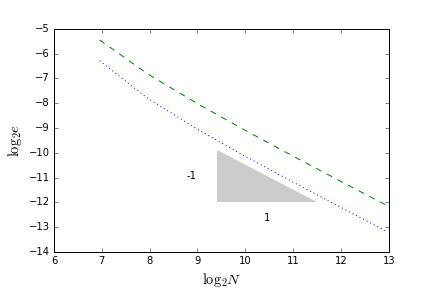
\includegraphics[scale=.5]{figures/convergenceVerification.png}
	\captionof{figure}{Numerical verification of the order of convergence of the error due to the Domain Decomposition Method \label{fig:orderVerification}}
\end{center}

\subsubsection{Corrections for the approximate TBCs}

\indent Then, we will formulate modified TBCs for the ASM method in order to cancel these errors :

\begin{equation}
    \begin{cases}
        \Theta_1^{c_L^*}(u_2^{n+1,k+1},0) + \theta_1 = \Theta_1^{c_L^*}(u_1^{n,k},0) + \theta_1' \\
        \Theta_2^{c_R^*}(u_1^{n+1,k+1},0) + \theta_2 = \Theta_2^{c_R^*}(u_2^{n,k},0) + \theta_2' \\
        \Theta_3^{c_R^*}(u_1^{n+1,k+1},0) + \theta_3 = \Theta_3^{c_R^*}(u_2^{n,k},0) + \theta_3'
    \end{cases}
\end{equation}

\noindent with $\theta_i, \theta_i'$ derived below, after a numerical verification of the error produced by the DDM.


\paragraph{Determination of $\theta_1, \theta_1'$}

\indent Our objective is to write (\ref{eq:FDdiscretization}) in the point $x_{N}$ :

\begin{equation}
    \label{eq:FDdiscretizationN}
    \frac{u_{N}^* - \alpha_{N}^*}{\Delta t} + \frac{-\frac{1}{2}u_{N-2}^* + u_{N-1}^* - u_{N+1}^* + \frac{1}{2}u_{N+2}^* }{\Delta x ^3} = 0
\end{equation}

\indent Defining 

\begin{gather}
    \theta_1 = c_L \frac{u_{N+1}^2 - u_{N}^2}{\Delta x} + c_L^2\frac{\Delta x}{\Delta t} \left( u_{N}^2 - \alpha_{N}^2 \right)\\
    \theta_1' = c_L \frac{u_{N}^1 - u_{N-1}^1}{\Delta x} - c_L^2\frac{\Delta x}{\Delta t} \left( u_{N}^1 - \alpha_{N}^1 \right)
\end{gather}

\indent we have, in the convergence, that

\begin{equation}
\label{eq:modifiedTBC1}
\begin{aligned}
&& &    \Theta_1^{c_L}(u_N^*) + \theta_1 = \Theta_1^{c_L}(u_N^*) + \theta_1'\implies \\
&& \implies &    u_N^* - c_L \frac{u_{N+1}^* - u_N^*}{\Delta x} + c_L^2\frac{u_N^* - 2u_{N+1}^* + u_{N+2}^*}{\Delta x^2} + c_L \frac{u_{N+1}^* - u_{N}^*}{\Delta x} + c_L^2\frac{\Delta x}{\Delta t} \left( u_{N}^* - \alpha_{N}^* \right) = \\
&& & u_N^* - c_L \frac{u_{N}^* - u_{N-1}^*}{\Delta x} + c_L^2\frac{u_N^* - 2u_{N-1}^* + u_{N-2}^*}{\Delta x^2} + c_L \frac{u_{N}^* - u_{N-1}^*}{\Delta x} - c_L^2\frac{\Delta x}{\Delta t} \left( u_{N}^* - \alpha_{N}^* \right) \implies \\
 && \implies &    2c_L^2 \frac{-\frac{1}{2}u_{N-2}^* + u_{N-1}^* - u_{N+1}^* + \frac{1}{2}u_{N+2}^* }{\Delta x ^2}  +             2c_L^2\frac{\Delta x}{\Delta t} \left( u_{N}^* - \alpha_{N}^* \right) = 0 \implies \\
&& \implies &    \frac{u_{N}^* - \alpha_{N}^*}{\Delta t} + \frac{-\frac{1}{2}u_{N-2}^* + u_{N-1}^* - u_{N+1}^* + \frac{1}{2}u_{N+2}^* }{\Delta x ^3} = 0
\end{aligned}
\end{equation}

\noindent which corresponds to the discretization \eqref{eq:FDdiscretization} satisfied in $x_N$. 

\paragraph{Determination of $\theta_2, \theta_2'$}

\indent Based on \eqref{eq:diffEquations}, we define

\begin{equation}
\begin{gathered}
    \theta_2 = \frac{\Delta x}{\Delta t} c_R^2 (u_N^1 - \alpha_N^1) \\
    \theta_2' = -\frac{\Delta x}{\Delta t} c_R^2 (u_N^2 - \alpha_N^2)
\end{gathered}
\end{equation}

\indent Indeed, we then have, in the convergence

\begin{equation}
\label{eq:modifiedTBC2}
\begin{aligned}
&& &\Theta_2^{c_R}(u_N^*) + \theta_2 = \Theta_2^{c_R}(u_N^*) + \theta_2'\implies \\
&& \implies & u_N^* - c_R^2 \frac{u_N^* - 2u_{N-1}^* + u_{N-2}^*}{\Delta x^2} + \frac{\Delta x}{\Delta t} c_R^2 (u_N^* - \alpha_N^*)  = \\ && & u_N^* - c_R^2 \frac{u_N^* - 2u_{N+1}^* + u_{N+2}^*}{\Delta x^2} -\frac{\Delta x}{\Delta t} c_R^2 (u_N^* - \alpha_N^*) \implies \\
&& \implies & 2\frac{\Delta x}{\Delta t} c_R^2 (u_N^* - \alpha_N^*) + 2c_R^2 \frac{-\frac{1}{2}u_{N-2}^* + u_{N-1}^* - u_{N+1}^* + \frac{1}{2}u_{N+2}^* }{\Delta x^2} = 0  \implies \\
&& \implies &\frac{u_N^* - \alpha_N^*}{\Delta t} + \frac{-\frac{1}{2}u_{N-2}^* + u_{N-1}^* - u_{N+1}^* + \frac{1}{2}u_{N+2}^* }{\Delta x^3} = 0
\end{aligned}
\end{equation}

\noindent which corresponds to the discretization \eqref{eq:FDdiscretization} satisfied in $x_N$.


\paragraph{Determination of $\theta_3, \theta_3'$}

\indent Using \eqref{eq:modifiedTBC2} in \eqref{eq:TBCsIterOmega1B}, we get

\begin{equation}
-\frac{u_{N-1}^* - 2 u_{N}^* + u_{N+1}^*}{\Delta x} + 2c_R\Delta x\frac{u_N^* - \alpha_N^*}{\Delta t} = 0 
\end{equation}

\indent Now, our objective is to write \eqref{eq:FDdiscretization} in the point $x_{N-1}$ :

\begin{equation}
    \label{eq:FDdiscretizationNm1}
    \frac{u_{N-1}^* - \alpha_{N-1}^*}{\Delta t} + \frac{-\frac{1}{2}u_{N-3}^* + u_{N-2}^* - u_{N}^* + \frac{1}{2}u_{N+1}^* }{\Delta x ^3} = 0
\end{equation}

\noindent what can be achieved by defining

\begin{equation}
\begin{gathered}
    \theta_3 = 2\frac{\Delta x}{\Delta t} \left[-\Delta x(u_{N-1}^1 - \alpha_{N-1}^1) - c_R (u_N^1 - \alpha_N^1) \right] + \frac{u_{N-3}^1 - 2u_{N-2}^1 + u_{N-1}^1}{\Delta x} \\
    \theta_3' = 0
\end{gathered}
\end{equation}

\indent In fact, in the convergence,

\begin{align*}
\label{eq:modifiedTBC3}
&&  &\Theta_3^{c_R}(u_N^*) + \theta_3 = \Theta_3^{c_R}(u_N^*) + \theta_3'     \implies \\
&& \implies & \frac{u_N^* - u_{N-1}^*}{\Delta x} + c_R \frac{u_N^* - 2u_{N-1}^* + u_{N-2}^*}{\Delta x^2} + 2\frac{\Delta x}{\Delta t}  \left[-\Delta x(u_{N-1}^* - \alpha_{N-1}^*) - c_R (u_N^* - \alpha_N^*) \right] + \\
&&   & 			\frac{u_{N-3}^* - 2u_{N-2}^* + u_{N-1}^*}{\Delta x}  =  \frac{u_{N+1}^* - u_{N}^*}{\Delta x} + c_R \frac{u_N^* - 2u_{N+1}^* + u_{N+2}^*}{\Delta x^2} \implies \\
&&  \implies &  -\frac{u_{N-1}^* - 2 u_{N}^* + u_{N+1}^*}{\Delta x} + 2c_R\Delta_x\frac{u_N^* - \alpha_N^*}{\Delta t} + \\
&&   & 2\frac{\Delta x}{\Delta t} \left[-\Delta x(u_{N-1}^* - \alpha_{N-1}^*) - c_R(u_N^* - \alpha_N^*) \right] + \frac{u_{N-3}^* - 2u_{N-2}^* + u_{N-1}^*}{\Delta x} = 0 \implies \\
&& \implies  & -2\frac{-\frac{1}{2}u_{N-3}^* + u_{N-2}^* - u_{N}^* + \frac{1}{2}u_{N+1}^* }{\Delta x} - 2\frac{\Delta x^2}{\Delta t}(u_{N-1}^* - 					\alpha_{N-1}^*) = 0 \implies \\
&& \implies &  \frac{u_{N-1}^* - \alpha_{N-1}^*}{\Delta t} + \frac{-\frac{1}{2}u_{N-3}^* + u_{N-2}^* - u_{N}^* + \frac{1}{2}u_{N+1}^* }{\Delta x ^3} = 0
\end{align*}

\paragraph{Modification of the reference solution}

\indent The modifications proposed above for the CBCs effectively allows the points $x_{N-1},x_N \in \Omega_1$ and $x_N \in \Omega_2$ to satisfy the same discrete equation as in the monodomain problem. Nevertheless, the solution of the DDM does not converge exactly to $u^{ref}$, for a reason that does not depend on the expression of the CBCs, but on the fact that for each domain we write two CBCs in the left boundry and only one on the right. We are using a second order centered discretization for the third spatial derivative (which uses a stencil of two points in each side of the central point), which implies that we must write an uncentered discretization for the point $x_{N+1}$ when solving the problem in $\omega_2$. Therefore, this point does not satisfy the same discrete equation. In order to avoid this problem and allow us to verify that our method is able to correct the error of the DDM, we modify the discretization for the point $u_{N+1}$ in the monodmoain problem, using the same second-order uncentered expression 

\begin{equation}
    \label{eq:uncenteredFDdiscretizationN}
    \frac{u_{N+1}^2 - \alpha_{N+1}^2}{\Delta t} + \frac{-\frac{5}{2}u_{N+1}^2 + 9u_{N+2}^2 - 12 u_{N+3}^2 + 7\frac{1}{2}u_{N+4}^2 -\frac{3}{2}u_{N+1}^2}{\Delta x ^3} = 0
\end{equation}

\subsection{Optimization of the CBCs (speed of convergence)}

\indent Our objective now is to optimize the CBCs in the sense of minimizing the number of iterations of the ASM until the convergence. Therefore, similarly to the optimization of the TBCs made in the section \ref{sec:TBC}, we will made a very large set of tests in order to find the coefficients $c_L$ and $c_R$ (i.e., the constant polynomial approximation for the TBC) that provides the fastest convergence. In a first moment, we will make this study with fixed time step and space step, in order to analyze exclusively the influence of the coefficient, and after we will introduce these two parameters into the study.

\indent As we are interested in the speed with which the solution of the DDM method converges to the reference solution, the criteria of convergence used is

\begin{equation}
\label{eq:criteriaConvergence}
	e^k = ||\tilde{u}^{k,DDM} - \tilde{u}^{k,ref}||_2 = \sqrt{\Delta x \left[ \sum_{j=0}^{N}{\left(u^{k,1}_j - u^{k,ref}_j \right)^2} + \sum_{j=N}^{2N}{\left(u^{k,2}_j - u^{k,ref}_j \right)^2} \right]} 
\end{equation}

\FloatBarrier
\bibliography{../may/biblio}

\end{document}